\cotefile{157-1}
\scanpage{242}

% top edge, circled manuscript number
\mspage{\textcircled{98}}

% whole-sheet schema, upper left to lower centre
{\scriptsize
\diagram{\begin{tikzcd}[ampersand replacement=\&,column sep=0.7em,row sep=3.7em,scale=0.60,transform shape,cells={nodes={inner sep=1pt}},every label/.append style={font=\tiny}]
{\left\{\begin{gathered}
\mathrm{Top}\,X\\
\text{loc. tot. 0-connexe}\\
\text{et 0 connexe}\\
\Leftrightarrow\text{ \unsure{tot.|tout} 0-connexe}\\
\text{et loc. irréd.}\\
\Leftrightarrow X\ \text{\uline{cofiltrante}}\\
\text{i.e. }\mathrm{PS}^{*}\unsure{1'|1}+\mathrm{PS}^{*}2\\
\Leftrightarrow X\ \text{0-connexe}\\
\unsure{+|*}\mathrm{PS}^{*}1+\mathrm{PS}^{\unsure{*|'}}2\\
\Leftrightarrow\left\{\begin{gathered}\forall x\in\mathrm{ob}\,X,\ X_{/x}\ \text{et}\\
X_{/x\times x}\text{ sont irréd.,}\\X\text{ 0-connexe}\end{gathered}\right.\\
\Leftrightarrow\left\{\begin{gathered}X\text{ 0-connexe,}\\
\text{les }X_{/a\times b}\text{ non vides (et }\Rightarrow\text{ 0-connexes)}\\
\text{les }X_{/a\times_{c} b}\text{ 0-connexes}\end{gathered}\right.
\end{gathered}\right.}
\arrow[rr,Rightarrow,"\substack{\mathrm{str.}\\{}[\mathrm{ex}\ \bullet\ \bullet]}"]
\arrow[d,Rightarrow,"\substack{\text{\uline{str.}}\ [\mathrm{ex}\mathord{:}\\B_G]}"']
\arrow[drr,Rightarrow,"\substack{\mathrm{str.}\\{}[\mathrm{ex.}\ \triangle]}"]
\& {\substack{\left[\begin{gathered}\text{stable par}\\\text{passage}\\\text{à }X'\longrightarrow X\\
\text{étale sur }X\text{ si}\\X'\text{ 0-connexe,}\\
\text{\uline{mais} si les}\\ X_{/a}\text{ sont cofiltrants}\\
\text{et }X\text{ \unsure{connexe},}\\\text{cela n'implique}\\
\text{\uuline{pas} }X\text{ cofiltrante}\end{gathered}\right]\\
\mathrm{Ex.}\ B_G}}
\& {\begin{gathered}
\text{\textcircled{\(\unsure{\varepsilon|e}=\bullet\ \bullet\)}}\\
\mathrm{Top}\,X\text{ loc. tot. 0-connexe}\\
\Leftrightarrow\text{ les comp. conn. de }X\\
\text{sont cofiltrantes}\\
\Leftrightarrow \mathrm{PS}^{*}1+\mathrm{PS}^{*}2\\
(X\ \text{\uline{loc. cofiltrante}})\\
\left[\begin{gathered}\text{stable par passage à }X'\longrightarrow X\\
\text{étale, mais si les }X'_{/x}\\
\text{y }\deleted{\text{\unsure{sont}}}\text{ satisfont, pas}\\
\text{forcément }X\unsure{!|^{\prime}!}\end{gathered}\right]
\end{gathered}}\arrow[dr,Rightarrow]\&\\
{\begin{gathered}\mathrm{Top}(X)\text{ loc. irréd }+\text{ 0-conn.}\\
\Updownarrow\\X\ \text{\uline{pseudofiltrante} }+\text{ \uline{0-connexe}}\\
\text{i.e. }\mathrm{PS}^{*}1+ \text{0-connexe}\\
\text{\textcircled{\(B_G\)}}
\end{gathered}}
\arrow[dr,Rightarrow,"\substack{\mathrm{str.}\\(\deleted{\mathrm{\unsure{ex}}}\mathord{:}\ 0\rightrightarrows1\unsure{)\!_{/*}|)}\\\deleted{\unsure{B_G}}}"']
\& {\left[\begin{gathered}\mathrm{PS}^{*}1\text{ ne dépend}\\
\text{que des catégories}\\\text{\unsure{induites|induites sur} }X_{/x}\\
\text{donc stable par passage}\\\text{aux }X'\longrightarrow X\text{ étales}\\
\text{donc la condition}\\\mathrm{PS}^{\unsure{*|'}}1+\text{0-conn stable}\\
\text{par passage aux rev.}\\X'\longrightarrow X\ \text{\uline{0-connexes}}\end{gathered}\right]}
\& {\begin{gathered}\mathrm{Top}\,X\ \text{\unsure{tot.} 0-connexe}\\
(\text{on dit }X\ \text{\uline{\unsure{tot.|tot.\,x} 0-connexe}}).\\
\Updownarrow\\X^{\circ}\longrightarrow X^{\circ}\times X^{\circ}\ \text{est \unsure{cofinal|cofinale}}\\
\text{\uline{et} }X^{\circ}\ne\varnothing\\
\Updownarrow\\
\left\{\begin{gathered}\forall x,y\in\mathrm{Ob}\,X,\quad x\times y\text{ 0-conn. ds }X^\wedge\\
\text{i.e. }X_{/x\times y}\text{ 0-conn.}\\
\deleted{\text{\unsure{et}}}\\\text{\uline{et} }X\ne\varnothing\end{gathered}\right.\\
*\ \text{\uline{Ex}}\ \text{\textcircled{\(\triangle\)}}\quad
\left[\begin{gathered}\text{NB n'est pas stable par}\\
\text{passage aux }X_{/x}^{*},\text{ et si}\\
\text{les }X_{/x}\text{ sont tot. 0-conn., }\inserted{\text{et }X\ne\varnothing,}\\
\text{il ne s'ensuit pas que}\\
\deleted{\text{\unsure{l'on}}}\ X\text{ le soit}^{**}\end{gathered}\right]\\
**\ \text{\uline{Ex}}\ B_G
\end{gathered}}
\arrow[dl,Rightarrow,"\substack{\mathrm{str.}\ [\mathrm{ex}\mathord{:}\ B_G\unsure{\amalg|\coprod},\ \text{ou}\\0\rightrightarrows1\ ]}"]
\&{\bigg\backslash\,\substack{\mathrm{Top}\,X\\\text{loc. irréd}}}\\
\&{\begin{gathered}
\mathrm{Top}\,X\text{ irréductible}\\
(X\ \text{\uline{irréductible}})\\
\Updownarrow\\ \mathrm{PS}^{*}1'
\end{gathered}}\&
\end{tikzcd}}}

% right of middle-right equivalence, delimited by an oblique stroke
% slanted delimiting stroke; words horizontal
% Right-hand marginal node transcribed at its arrowhead in the schema.

% below irreducibility node, bracket, first lines
[ne dépend que $\mathrm{Ord}\,X$ ou de $\mathrm{Esp}(X)$, signifie que $\mathrm{Ord}\,X$ cofiltrant, ou $\mathrm{Esp}(X)$ irréductible. N'est point stable par passage à $X'\longrightarrow X$ étales 0-connexes, p.ex. par passage à un $X_{/x}$, p.ex. $\inserted{X=}(0\rightrightarrows1)$ est irréd., mais $X_{/1}={}$(

% inside bracket, two arrows converging
\diagram{\begin{tikzcd}[ampersand replacement=\&,column sep=tiny,row sep=tiny]
\cdot\arrow[dr]\&\\[-1ex]\&\cdot\\[-1ex]\cdot\arrow[ur]\&
\end{tikzcd}}

% end of bracket
) ne l'est pas.]

% lower left, circled example
\margin{\textcircled{\(0\rightrightarrows1\)}}

% printed letterhead, inverted relative to manuscript, crossed by oblique pen strokes
% letterhead
\deleted{MINISTERE DE L'EDUCATION NATIONALE\\
ACADEMIE D'AIX-MARSEILLE\\
\rule{2em}{.3pt}\\
Inspection Académique\\
de Vaucluse\\
\rule{2em}{.3pt}\\
Tél. : 90 82 99 76\\
Référence : Secrétariat n\textsuperscript{o}}

% inverted letterhead, right column
% letterhead
\deleted{AVIGNON, le\\
L'Inspecteur d'académie,\\
directeur des services départementaux\\
de l'Education Nationale de Vaucluse,\\
à M}

% small pen trials between the printing, lower centre
\handwritten{\deleted{\unsure{A}}\quad\deleted{\illegible{1}}\quad\deleted{\unsure{Ai}}}

% bottom edge, left pen diagram
\handwritten{\deleted{\diagram{\begin{tikzcd}[ampersand replacement=\&,column sep=small,row sep=small]
y\arrow[r]\&\cdot\\
\cdot\arrow[r]\arrow[u]\&z\arrow[u]
\end{tikzcd}}}}

% bottom edge, right pen diagram
\handwritten{\deleted{\diagram{\begin{tikzcd}[ampersand replacement=\&,column sep=small,row sep=small]
\cdot\arrow[r]\& x\times x\\
\unsure{\int|f}\arrow[r]\arrow[u]\&\unsure{\bullet|x}\arrow[u]
\end{tikzcd}}}}

% archive sheet number: 242
\scanpage{243}

% top, circled number; archive foliation at upper left
\mspage{\textcircled{98}}

% upper schema, three middle nodes and one common bottom node
{\scriptsize\diagram{\begin{tikzcd}[ampersand replacement=\&,column sep=small,row sep=large,scale=.76,transform shape]
\&{\substack{\mathrm{Top}\,X\text{ loc. tot. 0-connexe}\\+\text{ 0-connexe}\\
(X\ \text{\uline{cofiltrante}})}}\arrow[dl,Rightarrow]\arrow[d,Rightarrow]\arrow[r,Rightarrow]\arrow[r,phantom,shift left=3ex,"\deleted{\Longrightarrow}"]
\&{\substack{\text{\textcircled{\(\unsure{\varepsilon|e}=\bullet\ \bullet\)}}\\
\mathrm{Top}\,X\text{ loc. tot. 0-conn.}\\(X\ \text{\uline{loc. cofiltrante}})\\
\mathrm{PS}^{*}1+\mathrm{PS}^{*}2}}\arrow[d,Rightarrow]\\
{\substack{\mathrm{Top}\,X\text{ loc. irréd }+\text{ 0\deleted{\unsure{c}}-conn}\\
(X\ \text{\uline{ps-filtrante} et \uline{0-connexe}})\\
\mathrm{PS}^{*}1+\text{0-connexe}\\ \text{\textcircled{\(B_G\)}}}}\arrow[dr,Rightarrow]
\&{\substack{\mathrm{Top}(X)\text{ tot. 0-conn,}\\(X\ \text{\uline{tot 0-conn.}})\\
X^\circ\longrightarrow X^\circ\times X^\circ\ \text{cofinal}\\
\text{\textcircled{\(\triangle\)}}}}\arrow[d,Rightarrow]
\&{\substack{\mathrm{Top}\,X\text{ loc. irréductible}\\
(X\ \text{\uline{\deleted{\unsure{ps-filtratif}}\unsure{ps-filtrante|ps-filtrative}}})\\
\mathrm{PS}^{*}1\\ \text{\tikz[baseline=(v.base)]{\node[draw,ellipse,inner xsep=2pt,inner ysep=1pt] (v) {\(\substack{B_G\amalg e\\\text{\unsure{ou|où} }G\ne1}\)};}}\quad\deleted{\text{\unsure{catégorie discrète}}}}}\\
\&{\substack{\mathrm{Top}(X)\text{ irréductible}\\(X\ \text{\uline{irréductible}})\\
\mathrm{PS}^{*}1'\\\text{\textcircled{\(0\rightrightarrows1\)}}}}\&
\end{tikzcd}}}

% middle right, NB underlined
\uline{NB} Les cinq catégories typiques $B_G$ $(G\ne1)$, $\triangle$, $0\rightrightarrows1$, $\varepsilon=\substack{\bullet\\[-.6ex]\bullet}$, $B_G\amalg e$ $(G\ne1)$ sont telles qu'elles appartiennent à la classe \unsure{envisagée} \inserted{$\unsure{C|\mathcal C}$} d'objets de Cat, mais à aucune \deleted{\unsure{classe autre}} des cinq autres classes sauf celles qui sont reliées à $C$ par $C\Rightarrow C'$ sur le diagramme d'implications (ou par une implication composée)

% middle left, unfinished line headed PS 1
\diagram{\begin{tikzcd}[ampersand replacement=\&,column sep=small,row sep=tiny]
\&\&b\&\\[-1ex]\text{\uline{PS 1}}\&\forall\ {\unsure{\bullet|a}}\arrow[ur]\arrow[dr]\&\&\exists\quad.\\[-1ex]\&\&c\&
\end{tikzcd}}

% lower schema, six classes and their examples
{\scriptsize\diagram{\begin{tikzcd}[ampersand replacement=\&,column sep=small,row sep=large,scale=.76,transform shape]
\&{\substack{X\ \text{\uline{cofiltrante}}\\ \mathrm{PS}^{*}1'+\mathrm{PS}^{*}2\\
=\mathrm{PS}^{*}1+\mathrm{PS}^{*}2+\text{0-conn}}}
 \arrow[dl,Rightarrow]\arrow[d,Rightarrow]\arrow[dr,Rightarrow]\&\\
{\substack{\text{\textcircled{\(B_G\)}}\quad X\ \text{\uline{\unsure{ps-cofiltrante|ps-filtrante}}}\\
\text{\uline{0-connexe}}\ \big|\ \mathrm{PS}^{*}1+\text{0-conn.}}}
 \arrow[dr,Rightarrow]\arrow[drr,Rightarrow,crossing over]
\&{\substack{X\ \text{\uline{tot. 0-conn}}\\
(X^\circ\longrightarrow X^\circ\times X^\circ\ \text{cofinal})\\
\text{\textcircled{\(\triangle\)}}}}\arrow[d,Rightarrow]
\&{\substack{\text{\textcircled{\(\bullet\ \bullet\)}}\\
X\ \text{\uline{loc. cofiltrante}}\\\mathrm{PS}^{*}1+\mathrm{PS}^{*}2}}\arrow[d,Rightarrow]\\
\&{\substack{X\ \text{\uline{irréductible}}\\ \mathrm{PS}^{*}1'\\
\text{\textcircled{\(\bullet\rightrightarrows\bullet\)}}}}
\&{\substack{X\ \text{\uline{pseudo-cofiltrante}}\\ \mathrm{PS}^{*}1\\
\text{\textcircled{\(B_G\amalg e\)}}}}
\end{tikzcd}}}

% bottom, first example
$\bullet\rightrightarrows\bullet$ n'est ni ps. cofiltrante, ni tot. 0-conn.

% bottom, second example
$B_G$ n'est ni loc. cofiltrante, ni tot. 0-conn

% bottom, third example, over cancelled criteria
$\triangle$ \deleted{$\mathrm{PS}^{*}1\quad\mathrm{PS}^{*}1'\quad\mathrm{PS}^{*}2\quad\text{0-conn.}$} n'est pas pseudo-filtrante

% foot, last example and addition beneath
$B_G\amalg e$ n'est pas loc. cof., car $B_G$ ne l'est pas, ni n'appartient à une des 4 classes d'objets connexes. \inserted{Idem pour $\varepsilon=\substack{\bullet\\[-.6ex]\bullet}$}

% archive sheet number: 243
\scanpage{244}

% letterhead, left column in reading orientation, inverted on scan
% letterhead
MINISTERE DE L'EDUCATION NATIONALE\\
ACADEMIE D'AIX-MARSEILLE\\
\rule{2em}{.3pt}\\
Inspection Académique\\
de Vaucluse\\
\rule{2em}{.3pt}\\
Tél. : 90 82 99 76\\
Référence : Secrétariat n\textsuperscript{o}

% letterhead, right column in reading orientation
% letterhead
AVIGNON, le\\[1ex]
L'Inspecteur d'académie,\\
directeur des services départementaux\\
de l'Education Nationale de Vaucluse,\\[1ex]
à M

% archive sheet number: 244
\scanpage{245}

% top, slightly right of centre
\mspage{99}

% top half, six-node implication schema
{\scriptsize\diagram{\begin{tikzcd}[ampersand replacement=\&,row sep=large,column sep=small,scale=.80,transform shape]
\&{\substack{X\ \text{\uline{cofiltrante}}\\
(\mathrm{PS}^{*}1'+\mathrm{PS}^{*}2\\ \deleted{\Leftrightarrow}\ \unsure{\mathrm{PS}^{*}1|{\mathrm{PS}}}\,1+\mathrm{PS}^{*}2+\text{0-conn})}}
\arrow[dl,Rightarrow]\arrow[d,Rightarrow,"\substack{\deleted{\unsure{\Rightarrow|\mathrm{PS}}}\mathrm{PS}^{*}1'\\(\Rightarrow\text{0-conn})}"']
\arrow[dr,Rightarrow,"\substack{\mathrm{PS}^{*}1\\(\text{les }{}_{a\backslash}X\text{ satisfont}\\ \mathrm{PS}^{*}1')}"']
\&\\
{\substack{\text{\textcircled{\(\triangle\)}}\quad X\text{ tot 0-conn}\\(X^\circ\to X^\circ\times X^\circ\ \text{cofinal})}}\arrow[d,Rightarrow]
\&{\substack{X\ \text{\uline{\unsure{pscofiltrante|pseudofiltrante|pscofiltrant}}}\\\text{0-connexe}\\(\mathrm{PS}^{*}1+\text{0-conn.})\\(\text{manque }\mathrm{PS}^{*}2)\\\text{\textcircled{\(B_G\)}}\\G\ne\{1\}}}\arrow[dl,Rightarrow]\arrow[dr,Rightarrow]
\&{\substack{\text{\textcircled{\(\unsure{\varepsilon|e}=\substack{\bullet\\[-.65ex]\bullet}\)}}\\
\underbrace{(\text{\unsure{comp.|compos.} conn. filtrantes})}\\X\ \text{\uline{loc. cofiltrante}}\\
(\mathrm{PS}^{*}1+\mathrm{PS}^{*}2)}}\arrow[d,Rightarrow]\\
{\substack{X\text{ irréductible}\\(\mathrm{PS}^{*}1')\\
\text{\textcircled{\(\bullet\rightrightarrows\bullet\)}}}}
\&\&{\substack{\underbrace{(\text{comp. conn. ps. filtrantes})}\\
X\ \text{\uline{pseudo-cofiltrante}}\\ \text{ou encore \uline{loc. irréductible}}\\
(\mathrm{PS}^{*}1.)\\ \text{\textcircled{\(B_G\amalg e\)}}\\G\ne\{1\}}}
\end{tikzcd}}}

% centre above second schema
et dualement on a $\downarrow$

% lower half, six-node dual schema
{\small\diagram{\begin{tikzcd}[ampersand replacement=\&,row sep=large,column sep=small,scale=.80,transform shape]
\&{X\ \text{\deleted{co}filtrante}}\arrow[dl,Rightarrow]\arrow[d,Rightarrow]\arrow[dr,Rightarrow]\&\\
{X^\circ\text{ tot. 0-connexe}}\arrow[d,Rightarrow]\&
{\substack{X\text{ ps-filtrante}\\\text{0-conn.}}}\arrow[dl,Rightarrow]\arrow[dr,Rightarrow]\&
{X\text{ loc. filtrante}}\arrow[d,Rightarrow]\\
{X\text{ coirréductible}}\&\&{X\text{ ps-filtrante}}
\end{tikzcd}}}

% below dual schema, left
donc on a une terminologie \unsure{décente|directe} sauf pour ``$X^\circ$ tot. 0-connexe'' -- je n'ose dire ``$X$ \unsure{tot.|dét.} co-connexe''!!

% inverted printed letterhead, left column when upright
% letterhead
\deleted{MINISTERE DE L'EDUCATION NATIONALE\\
ACADEMIE D'AIX-MARSEILLE\\
\rule{2em}{.3pt}\\
Inspection Académique\\
de Vaucluse\\
\rule{2em}{.3pt}\\
Tél. : 90 82 99 76\\
Référence : Secrétariat n\textsuperscript{o}}

% inverted printed letterhead, right column when upright
% letterhead
\deleted{AVIGNON, le\\
L'Inspecteur d'académie,\\
directeur des services départementaux\\
de l'Education Nationale de Vaucluse,\\
à M}

% bottom left over the letterhead, two outlines joined by diagonals
\handwritten{\figure{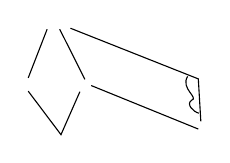
\begin{tikzpicture}[x=.8cm,y=.65cm]
\draw (0,1.15)--(.3,2.1) (.5,2.1)--(.9,1.12) (1,1)--(2.7,.15) (.67,2.12)--(2.7,1.13)--(2.74,.3) (0,.89)--(.52,.04)--(.82,.88);
\draw (2.53,1.18) .. controls (2.41,.94) and (2.72,.76) .. (2.59,.71) .. controls (2.5,.63) and (2.63,.48) .. (2.71,.46);
\end{tikzpicture}}}

% bottom centre-right, three uprights connected by sloping lines
\handwritten{\figure{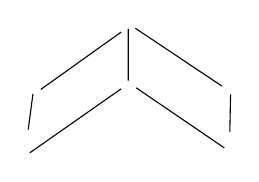
\begin{tikzpicture}[x=1cm,y=.7cm]
\draw (0,.45)--(.06,1.1) (.16,1.18)--(1.18,2.22) (1.27,2.28)--(1.27,1.34) (1.36,2.29)--(2.46,1.24) (2.57,1.09)--(2.56,.41) (1.37,1.21)--(2.49,.12) (1.18,1.19)--(.02,.03);
\end{tikzpicture}}}

% archive sheet number: 245
\scanpage{246}

% entire draft, rotated 180 degrees for reading; two long cancellation strokes
\deleted{

% top four definitions and braces
\[
\begin{aligned}
\mathrm{PS}^{*}1'\deleted{\unsure{*|1}}&\quad\text{catégorie irréductible}\\
\mathrm{PS}^{\deleted{*}}1'&\quad\text{catégorie co-irréductible}\\[-.3ex]
&\quad\left.\vphantom{X^X}\right\}\ \text{Ne dépend que de }\mathrm{Ord}\,X\\
\mathrm{PS}^{*}1\deleted{\unsure{'|*}}&\quad\text{Catégorie loc. irréductible}\\
&\quad\inserted{\text{ou pseudo-cofiltrante}}\\
\mathrm{PS}\,1&\quad\text{Catégorie coloc. co-irréductible}\\
&\quad\underbrace{\hphantom{\text{coloc. co-irréductible}}}_{\text{pseudo-filtrante}}\\
&\quad\left.\vphantom{X^X}\right\}\ \text{Ne dépend que des }X_{/\unsure{a|x}}\ \text{resp. }{}_{a\backslash}X
\end{aligned}
\]

% upper middle, equivalence and underbrace
\[
\underbrace{\mathrm{PS}\,1+\mathrm{PS}\,2+\text{0-conn}\ \Leftrightarrow\
\mathrm{PS}'1+\mathrm{PS}\,2}_{\text{\unsure{Cat\textsuperscript{e}|Cat\textsuperscript{n}} filtrante}}
\]

% right of equivalence, separated by oblique line
% slanted
\margin{$X$ cofiltrante $\Rightarrow$ \deleted{les \unsure{$X$}} tous $X'$ étales sur $X$ cof., donc les $X_{/a}$ cofiltrants. \uline{mais} \uline{réciproque} \uline{\unsure{faux|fausse}}}

% middle left, isolated sum
\[\mathrm{PS}^{*}\unsure{1|1'}+\mathrm{PS}^{*}2\]

% middle, ordinal and spatial criteria
{\scriptsize\diagram{\begin{tikzcd}[ampersand replacement=\&,column sep=1.2em,row sep=small]
\&\&{\mathrm{Ord}\,X\text{ cofiltrant}}\arrow[d,Leftrightarrow]\\
{X\text{ irréductible}}\arrow[r,Leftrightarrow]\&{\mathrm{Top}(X)\text{ irréd}}\arrow[r,Leftrightarrow]\&
{\mathrm{Esp}(X)\text{ irréd}}\\
{X\text{ coirréductible}}\arrow[r,Leftrightarrow]\&{\mathrm{Top}(X^\circ)\text{ irréd.}}\arrow[r,Leftrightarrow]\&
{\mathrm{Esp}(X_{\unsure{o|\circ}})\text{ irréd}\ \Leftrightarrow\ \substack{\mathrm{Ord}\,X^\circ\\\text{cofiltr.}}}
\end{tikzcd}}}

% middle, second equivalence pair
\[
\begin{aligned}
X\ \text{ps-cofiltrante}\ \inserted{\text{(ou loc. irréductible)}} &\Leftrightarrow \text{les } X_{/a}\text{ sont irréductibles}\\
&(\Leftrightarrow \mathrm{Top}\,X\text{ loc irréd})\\
X\ \text{ps-filtrante} &\Leftrightarrow \text{les }{}_{a\backslash}X\text{ sont coirréductibles}\\
&(\Leftrightarrow\mathrm{Top}\,X^\circ\text{ loc irréd})
\end{aligned}\]

% below equivalences, opposite implications
\diagram{\begin{tikzcd}[ampersand replacement=\&,column sep=large]
{X\text{ irréductible}}\arrow[r,Rightarrow,shift left=1ex,"{\diagup}" description]
\&{X\text{ ps.cofiltrante }\deleted{\text{0-connexe}}}\arrow[l,Rightarrow,shift left=1ex,"{\deleted{\diagup}}" description]
\end{tikzcd}}

% lower middle, parallel-arrow example
$0\,\bullet\rightrightarrows\bullet\,1$ est irréductible mais non ps. cofiltrante car $X_{/1}={}$

% end of line, three-point diagram
\diagram{\begin{tikzcd}[ampersand replacement=\&,column sep=tiny,row sep=tiny]
\cdot\arrow[dr]\&\\[-1ex]\&\cdot\\[-1ex]\cdot\arrow[ur]\&
\end{tikzcd}}

% below example
n'est pas cofiltrante.

% bottom left, isolated vertically curved arrow and unlabelled arrow network
\diagram{\begin{tikzcd}[ampersand replacement=\&,column sep=1ex,row sep=.75ex]
{}\&\&\&{}\arrow[dr]\&\\
\cdot\arrow[u,bend left]\&\&{}\arrow[ur]\arrow[dr]\&\&{}\\
\&{}\arrow[ur]\arrow[dr]\&\&{}\arrow[ur]\arrow[dr,dash]\&\\
\&\&{}\arrow[ur]\&\&{}\\
\&\&\&{}\arrow[ul,leftrightarrow]\arrow[ur,very thick]\&
\end{tikzcd}}

% bottom right, three descending conditions
\diagram{\begin{tikzcd}[ampersand replacement=\&,row sep=1em]
\&X\text{ filtrante}\arrow[d,Rightarrow]\\
{\text{0-conn}+\mathrm{PS}\,1}\&{X\ \underbrace{\text{ps\deleted{\unsure{f}}filtrant}}_{\mathrm{PS}\,1}\ \text{0-connexe}}\arrow[d,Rightarrow]\\
{\unsure{\mathrm{PS}+1'|\mathrm{PS}\,1'}}\&{X\text{ coirréductible}\quad(\mathrm{PS}\,1')}
\end{tikzcd}}

% close whole-sheet cancellation
}

% archive sheet number: 246
\scanpage{247}

% upper face, two-line pencil title
\unsure{Kan} \unsure{extensions|extension} dans les dérivateurs

% right of title, numeral with upper and lower rules
$\overline{\underline{\mathrm{III}}}$

% archive sheet number: 247
\scanpage{248}

% top, heading and small number above it
\mspage{1}Relations des dérivateurs avec la catégorie Hot.

% lines 2–3
Soit $\mathbb D$ un dérivateur, $\mathcal A$ sa catégorie fondamentale

% line 3, centred
\[\mathcal A=\mathbb D(e)\]

% lines 4–5
Je me propose de définir, \deleted{\unsure{dès}} \unsure{si} faire se peut, des foncteurs

% upper display (1), under one left brace, with right-hand formulas
\[
\left\{\begin{aligned}
\mathrm{Hot}\times\mathcal A&\xrightarrow{\pi_{\mathbb D}}\mathcal A
&(\unsure{\xi|\zeta}\,\unsure{,|\times}\,\deleted{\unsure{F|M}}\unsure{M|F})&\longrightarrow\xi\times F\ \text{ou }\xi\otimes\deleted{\unsure{F}}M\\
&&&\text{(suivant les cas)}\\
\mathrm{Hot}^{\circ}\times\mathcal A&\xrightarrow{\varpi_{\mathbb D}}\mathcal A
&(\xi,\deleted{\unsure{F}}\unsure{M|A})&\longrightarrow
\unsure{\mathrm{hom}|\mathrm{Hom}}(\xi,\deleted{\unsure{F}}M)
\end{aligned}\right.\tag*{(1)}
\]

% below (1), lines 1–3
Ces foncteurs doivent s'échanger par dualité : si on prend les foncteurs $\pi^\circ$, $\varpi^\circ$ sur les catégories opposées, on trouve

% middle display (1′)
\[
\left\{\begin{aligned}
\unsure{\mathrm{HOT}|\mathrm{Hot}}\times\mathcal A^\circ&\xrightarrow{\deleted{\varpi^\circ}\ \varpi_{\mathbb D}^{\circ}}\mathcal A^\circ\\
\mathrm{Hot}^{\circ}\times\mathcal A&\xrightarrow{\pi_{\mathbb D}^{\circ}}\mathcal A^\circ
\end{aligned}\right.\tag*{(\uline{1}')}
\]

% above duality identities
et on doit avoir

% middle, two identities and struck label
\[
\left\{\begin{aligned}
\varpi_{\mathbb D}^\circ&=\pi_{\mathbb D^\circ}\\
\deleted{\unsure{\varpi|\pi}}\pi_{\mathbb D}^\circ&=\varpi_{\mathbb D^\circ}
\end{aligned}\right.\ .\tag*{\deleted{\unsure{(2)}}}
\]

% line immediately below the identities
\deleted{\unsure{Les|Leurs} propriétés fondamentales}

% lower half, introduction to functor form
À vrai dire, considérant (1) comme des foncteurs

% lower half, first unnumbered pair
\[\begin{aligned}
\mathrm{Hot}&\xrightarrow{\pi_{\mathbb D}}\underline{\mathrm{Hom}}(\mathcal A,\mathcal A)\\
\mathrm{Hot}^{\circ}&\xrightarrow{\varpi_{\mathbb D}}\underline{\mathrm{Hom}}(\mathcal A,\mathcal A)
\end{aligned}\]

% before (2)
on s'attend à ce que ces foncteurs s'étendent en

% lower display (2)
\[
\left\{\begin{aligned}
\mathrm{Hot}&\xrightarrow{\pi_{\mathbb D}}\underline{\mathrm{Hom}}(\mathbb D,\mathbb D)\\
\mathrm{Hot}^{\circ}&\xrightarrow{\varpi_{\mathbb D}}\underline{\mathrm{Hom}}(\mathcal A,\mathcal A)
\end{aligned}\right.\tag*{(2)}
\]

% foot, last four lines with added qualification
Cela signifie, essentiellement, que \inserted{pour $\xi\in\mathrm{Ob}\,\mathrm{Hot}$ donné,} les opérations $\xi\times_{\mathbb D}M$ et $\underline{\mathrm{Hom}}_{\mathbb D}(\xi,F)$ sont définies non seulement dans $\mathcal A=\mathbb D(e)$, mais dans tous les $\mathbb D(I)$, et ceci de façon à commuter aux foncteurs $f^*$ :

% archive sheet number: 248
\scanpage{249}

% top number, word at upper left
\mspage{2}\unsure{Si|si}

% opening arrow
\[f:I'\longrightarrow I\]

% line beneath opening arrow
alors pour $F\in\mathrm{Ob}\,\mathbb D(I)$, on doit avoir des iso. can.

% (3), two restriction isomorphisms
\[
\left\{\begin{aligned}
f^{*}(\unsure{\xi|\zeta}\times_{\mathbb D}\unsure{M|F})&\simeq
\deleted{\unsure{f^{*}|\xi}}\deleted{\unsure{\xi}}\xi\times_{\mathbb D} f^{\unsure{'|*}}(M)\\
f^{*}\mathrm{Hom}_{\mathbb D}(\xi,M)&\simeq\mathrm{hom}(\xi,f^{*}(M))\ ,
\end{aligned}\right.\tag*{(3)}
\]

% below (3), two lines
avec les compatibilités habituelles pour un composé $fg$, \unsure{relatif},

% inline chain after relatif
\diagram{\begin{tikzcd}[ampersand replacement=\&]
I''\arrow[r,"g"]\&I'\arrow[r,"f"]\&I.
\end{tikzcd}}

% middle paragraph, four lines
Mais je me place de préférence dans $\mathcal A$, ce qui devrait impliquer les constructions simultanées dans tous les $\deleted{\unsure{\mathcal A}}\mathbb D(I)$, quitte à appliquer ce qui a été dit au dérivateur $\mathbb D_I$.

% middle, next two lines
L'intuition algébrique fondamentale est celle-ci, en désignant par

% localization functor
\[X\longrightarrow\mathrm{hot}(X):\quad(\mathrm{Cat})\longrightarrow(\mathrm{Hot})\]

% lower middle, localization and choice of X
le foncteur de localisation de (Cat) dans Hot, obtenu en inversant les flèches de (Cat) qui sont des ``équivalences faibles''. Supposons $X$ dans $\mathrm{Diag}$, soit \deleted{$\unsure{p}$}

% lower line, projection
\[p:X\longrightarrow e\]

% above (4), correction before à val.
\unsure{le|la} \deleted{\unsure{pro}}\deleted{\unsure{foncteur}}\deleted{\unsure{obtenu|structural}} à val. dans la cat. ponctuelle. On sent que

% (4), homology and cohomology formulas
\[
\left\{\begin{aligned}
\mathrm{hot}(X)\times_{\mathbb D}M&\simeq p_{\deleted{\unsure{*}}!}(p^{*}(M))
=H^{\unsure{\cdot\mathbb D|\mathbb D}}_{\deleted{\unsure{\mathbb D}}\bullet}(X,M)\\
\mathrm{Hom}_{\mathbb D}(\mathrm{hot}(\unsure{x|X}),M)&\simeq p_{\deleted{\unsure{!}}*}(p^{*}(M))
=H_{\mathbb D}^{\deleted{\unsure{\mathbb D}}\bullet}(X,M)
\end{aligned}\right.\tag*{(4)}
\]

% last line
(iso canoniques).

% archive sheet number: 249
\scanpage{250}

% head and opening, lines 1–5
\mspage{3}Ceci donnerait un principe de définition pour les opérations cherchées, Une difficulté vient du fait qu'en général, $\mathrm{Diag}$ n'est pas égal à (Cat), et que les types d'homotopie provenant de $\mathrm{Diag}$ ne \deleted{\unsure{sont}} \unsure{épuisent|forment|donnent} pas ($=$ à isom. près) \uline{tous} les types d'homotopie.

% upper middle, continuation and corrections, lines 6–11
\deleted{\unsure{Par} Mais on peut \unsure{se borner}} \inserted{Intuitivement, on} ne trouve que des types d'homotopie ``assez petits''. Mais on peut localiser $\mathrm{Diag}$ par ses \deleted{\unsure{qu}} \unsure{équ.|équi.} faibles (il \unsure{vaut|faut} mieux dire ``quasi-isomorphismes''), on trouve alors une catégorie \deleted{\unsure{plus}} $(\mathrm{Hot})_0$, et un foncteur canonique

% central arrow
\[\mathrm{Hot}_0\longrightarrow\mathrm{Hot}\ ,\]

% lower half, lines 1–7
si on a de la chance ce foncteur sera pleinement fidèle, et on \deleted{\unsure{défini}} essayera de décrire les foncteurs (1) ou (2) en y remplaçant Hot par la sous-catégorie pleine des ``petits'' types d'homotopie. On peut aussi oublier (provisoirement!) Hot, et travailler avec $\mathrm{Hot}_0$. C'est ce qu'on va faire pour le moment.

% before (5)
Pour pouvoir définir les foncteurs

% (5), product and Hom
\[
\left\{\begin{aligned}
\mathrm{Hot}_0^{\deleted{\unsure{\circ}}}\deleted{\unsure{\otimes}}\times\mathcal A&\longrightarrow\mathcal A&
(\unsure{\xi|\zeta}\unsure{\times|,} F)&\longmapsto\xi\times_{\mathbb D}F\\
\mathrm{Hot}_0^\circ\times\mathcal A&\unsure{-|\to}\mathcal A&
(\xi,F)&\longmapsto\mathrm{Hom}_{\deleted{\mathbb D}\mathbb D}(\xi,F)\ ,
\end{aligned}\right.\tag*{(5)}
\]

% foot, line carried over to next scan
je note que pour $F$ fixé, $X$ variable \deleted{\unsure{en}}dans $\mathrm{Diag}$, les

% archive sheet number: 250
\scanpage{251}

% head, continuation of scan 250
\mspage{4}\unsure{derniers|deuxièmes} mbs des (4)

% upper display with scratched left label
\[H^{\mathbb D}_{\bullet}(X,M),\quad H_{\mathbb D}^{\bullet}(X,M)\ ,\tag*{\deleted{\unsure{(6)}}}\]

% top paragraph following display, eight lines
sont bien, l'un covariant, l'autre contravariant en $X$. Donc il y a, à isom unique près, une seule paire de bifoncteurs (5) satisfaisant (bi)fonctoriellement des isom. (4), \unsure{ssi|si} les \deleted{foncteurs}\inserted{expressions} (6), considérées comme fonctorielles en $X$, transforment quasi-isomorphismes en isomorphismes. Cela équivaut donc à la validité du

% middle, theorem, two vertical strokes at left
\uline{Théorème} (\unsure{?|6}) Soit $f:X'\longrightarrow X$ dans $\mathrm{Diag}$. Si $f$ est un quasi-isom, c'est une $\mathbb D$-équivalence.

% left of theorem, written obliquely rising to the right
% slanted
\margin{Nouvel axiome ?}

% below theorem through middle of lower third
Quand $X$ \unsure{$\to$|est} la cat. ponctuelle, ce n'est \inserted{\unsure{là|l'}} autre que l'axiome Dér 3 (p. 67). \deleted{\unsure{Nous allons}} J'ignore si c'est une conséquence des axiomes Der 1 à der 5 (1). Si ce n'est pas le cas, il faudrait l'ajouter aux axiomes, je crois. Je n'ai pas même prouvé qu'une équiv. de catégories \inserted{$\in\mathrm{Diag}$} (au sens des catégories !) est une $\mathbb D$-équivalence !

% before (7)
Notons la \uline{formule d'adjonction}

% (7), adjunction
\[\mathrm{Hom}(\unsure{\xi|\zeta}\times_{\mathbb D}M,N)\unsure{\xrightarrow{\sim}|\simeq}
\mathrm{Hom}(M,\mathrm{hom}_{\mathbb D}(\xi,N))\tag*{(7)}\]

% between (7) and (8)
Si $\xi$ provient \deleted{\unsure{Hot}} de $X\in\deleted{\unsure{\mathcal C}}\mathrm{Diag}$, \unsure{donc|dès} cela s'écrit

% (8), last line
\[\mathrm{Hom}(p_!p^*M,N)\xrightarrow{\sim}\mathrm{Hom}(M,p_*p^{\unsure{'|*}}N)\ ,\tag*{(8)}\]

% archive sheet number: 251
\scanpage{252}

% head and first line
\mspage{5}or par adjonction les deux membres sont can. isom à

% opening Hom space
\[\mathrm{Hom}_{\mathbb D(X)}(p^*M,p^{\unsure{*|'}}N)\ .\]

% example, two lines above diamond
\deleted{\uline{Ex}} \uline{Ex} Prenant pour $\unsure{\xi|\zeta}$ le type d'homotopie du cercle \unsure{standard|standart} (représenté p.ex. par l'ens ordonné

% upper middle, four-object ordered set
\diagram{\begin{tikzcd}[ampersand replacement=\&,column sep=small,row sep=small]
\&b\&\\
\unsure{o|0}\arrow[ur]\arrow[dr]\&\&o'\arrow[ul]\arrow[dl]\\
\&a\&
\end{tikzcd}}

% text below diamond through cartésiens, including the interlinear additions
(où on convient de prendre $o$ comme origine, et d'orienter de $o$ en $a$), les deux foncteurs en question sont \inserted{(sauf erreur)} les foncteurs suspension $\Sigma$ et ``cosuspension'' ou ``\inserted{foncteur} \unsure{espaces|espace} des lacets'' $\Omega$. Je me réserve de vérifier que $\Omega F$ coïncide bien avec ce que j'ai décrit ailleurs, à propos des carrés \unsure{substantiels} cartésiens dans $\mathcal A$.

% lower middle, introduction of the product
Dans $\mathrm{Hot}_0$ on a une opération produit, en fait ça doit être le produit catégorique dans $\mathrm{Hot}_0$. Mais sans la \unsure{considérer|caractériser|vérifier} \deleted{\unsure{il}}elle est donnée par

% second formula labelled (8)
\[\unsure{\mathrm{hot}|\mathrm{Hot}}_0(X)\times\unsure{\mathrm{Hot}|\mathrm{hot}}_0(Y)\simeq\mathrm{hot}_0(X\times Y)\tag*{(8)}\]

% before (9), single line
Ceci posé, on a les iso. canoniques, pour $\xi,\unsure{\eta|y}\in\mathrm{Ob}\,\mathrm{Hot}^{\unsure{0|\circ}}$

% (9), two action identities
\[
\left\{\begin{aligned}
\xi\times_{\mathbb D}(\eta\times_{\mathbb D}M)&=(\xi\times\eta)\times_{\mathbb D}M\\
\mathrm{Hom}_{\mathbb D}(\xi,\mathrm{hom}_{\mathbb D}(\eta,M))&\simeq
\mathrm{hom}_{\mathbb D}(\xi\times\eta,M)
\end{aligned}\right.\tag*{(9)}
\]

% last line, continues overleaf
Si $\deleted{X}\xi,\eta$ sont représentés par $X,Y$, la première formule p.ex

% archive sheet number: 252
\scanpage{253}

% upper centre, folio
\mspage{6}

% upper left, square with diagonal
\diagram{\begin{tikzcd}[ampersand replacement=\&,column sep=small,row sep=small]
X\arrow[d,"p"']\&X\times_e Y\arrow[l,"q'"']\arrow[d,"p'"]\arrow[dl,dashed,"\varphi"']\\
e\&Y\arrow[l,"q"]
\end{tikzcd}}

% upper right, continuation from scan 252
s'établit en calculant le deuxième \unsure{mb|mbr} comme

% upper right, below continuation
\[
\varphi_!(M_{X\times Y})\simeq
p_!\bigl(\underbrace{q'_!(M_{X\times Y})}_{\substack{\rotatebox{90}{\(\simeq\)}\\q_!(M_Y)_X\\\text{car }q\text{ est}\\\mathbb D\text{-lisse}}}\bigr)
\simeq\unsure{\xi|\zeta}\times_{\mathbb D}(\unsure{\eta|y}\times_{\mathbb D}M)
\qquad\text{OK.}
\]

% before proposition
J'ai aussi envie de prouver

% proposition with interlinear hypothesis
\uline{Proposition !} \inserted{Soit $\xi\in\mathrm{Ob}\,\mathrm{Hot}_0$. Alors} $F\mapsto\xi\times_{\mathbb D}F$, en tant que morphisme de dérivateurs $\mathbb D\unsure{-|\to}\mathbb D$, est \uline{exact à droite}, et $F\mapsto\mathrm{hom}_{\mathbb D}(\xi,F)$ est exact à gauche.

% above middle display
\unsure{OBS} que $\xi$ est défini par $X$ dans $\mathrm{Diag}$. Soit $f:\deleted{\unsure{X|I}}I\longrightarrow J$, \deleted{\unsure{i|il}}soit $F$ dans $\mathbb D(I)$, il faut prouver

% middle, desired comparison
\[f_*(\mathrm{hom}_{\mathbb D}(\xi,F))\simeq \mathrm{Hom}_{\mathbb D}(\xi,f_*(F))\]

% above middle square
Considérons donc

% middle, comparison square
\diagram{\begin{tikzcd}[ampersand replacement=\&,column sep=large]
X\times I\arrow[r,no head,"f'"]\arrow[d,"p="',"{(x,i)\mapsto i}"]\& X\times J\arrow[d,"{q=(x,j)\mapsto j}"]\\
I\arrow[r,"f"]\&J
\end{tikzcd}}

% below square
On a

% first line below square
\[\mathrm{hom}_{\mathbb D}(\xi,F)=p_*(p^*F)\]

% between computations
donc

% composite direct images
\[f_*(\mathrm{hom}_{\mathbb D}(\xi,F))=\underbrace{f_*p_*}_{(fp)_*}(\unsure{y'|\gamma'|p'|p^*}F)\simeq(qf')_*p^*(F)\simeq q_*(f'_*p^*(F))\]

% above base-change formula
Mais

% base-change formula
\[f'_*p^*(F)\simeq q^*f_*(F)\]

% last three lines
formule de changemt de base des $f_*$, pour le chgt de base $q$, qui est lisse, car il dérive de $X\longrightarrow e$ qui est lisse par chgt. de base $J\longrightarrow e$. On trouve

% archive sheet number: 253
\scanpage{254}

% folio and opening word
\mspage{7}donc

% opening comparison
\[f_*(\mathrm{hom}_{\mathbb D}(\unsure{\xi|\zeta},F))\simeq q_*q^*(f_*(F))\overset{\mathrm{def}}{=}\mathrm{hom}_{\mathbb D}(\xi,f_*(F))\]

% below opening comparison
qed. L'énoncé pour $F\mapsto\xi\times_{\mathbb D}F$ est dual de celui qu'on vient de prouver.

% upper middle, before adjunction
Reprenons, pour $\xi\in(\mathrm{Hot})_0$, la formule d'adjonction

% adjunction, label left
\[\mathrm{Hom}(\xi\times_{\mathbb D}M,N)\simeq\mathrm{Hom}(M,\unsure{\mathrm{Hom}|\mathrm{hom}}_{\mathbb D}(\xi,N))\overset{\mathrm{def}}{=}\mathrm{Hom}_{\xi}(M,N)\tag*{\(\unsure{a|\alpha})\)}\]

% struck beginning immediately below adjunction
\deleted{Pour $M,N$ fixés, et}

% above Hom formula
Si $\xi$ est défini par $X$ dans $\mathrm{Diag}$, les deux \unsure{mbs|mbr} de (a) s'identifient à

% middle, Hom in the fibre
\[\mathrm{Hom}_{\mathbb D(X)}(p^*M,p^*N),\]

% middle, structural functor
où $p:X\longrightarrow e$ est le foncteur structural.

% middle, variable coefficient
Fixons $M,N$, et considérons l'expression (a) comme contrafoncteur

% target of contrafunctor
\[(\mathrm{Hot}_0)^{\unsure{\circ|0}}\longrightarrow\mathrm{Ens}\]

% bottom paragraph and inserted letter
Il semblerait que dans tous les cas connus, ce foncteur soit ``représentable'' par un objet, \unsure{sinon} de $\mathrm{Hot}_0$ lui-\unsure{m\textsuperscript{=}|même}, du moins \deleted{\unsure{un}}objet dans $\mathrm{Hot}$. \deleted{\unsure{Un}} Si \deleted{\unsure{l'|a}}on ne peut le définir comme objet \inserted{$H$} de $\mathrm{Hot}_0$, le fait qu'on ait un isom canonique

% bottom formula (10)
\[\mathrm{Hom}_{\xi}(M,N)\simeq\mathrm{Hom}_{\mathrm{Hot}}(\xi,H),\tag*{(10)}\]

% last line, continuing on 255
fonctoriel en $\xi\in\mathrm{Ob}\,\mathrm{Hot}_0$, ne définit pas \unsure{forcément}

% archive sheet number: 254
\scanpage{255}

% folio and opening continuation
\mspage{8}à isom unique près. En fait, quand

% derivator defined by a pair
\[\mathbb D=\mathbb D_{\deleted{\unsure{D|M}}\mathcal M,\Sigma}\]

% between first two displays
est défini par une catégorie de modèles $(\mathcal M,\Sigma)$, alors il y a une définition naturelle \deleted{de l'espèce} d'une opération $\mathrm{Hom\,ext}$ (Hom ``externe'') à valeurs en $\mathrm{Hot}$, \deleted{\unsure{dans $\mathcal A$}} savoir un foncteur

% display (11), two lines with a left brace
\[
\left\{\begin{aligned}
\mathcal A^{\unsure{\circ|0}}\times\mathcal A&\longrightarrow\mathrm{Hot}\\
(M,N)&\longmapsto\mathrm{Hom\,ext}(M,N)
\end{aligned}\right.\tag*{(11)}
\]

% after (11), fundamental category
où $\mathcal A=\mathcal M\Sigma^{-1}$ est la cat. fond. de $\mathbb D=\mathbb D_{\mathcal M,\Sigma}$.

% middle paragraph, verification and source
\deleted{\unsure{Quand} \illegible{1}} Il est vrai que je n'ai pas vérifié que \deleted{\unsure{si|a}}si p.ex. $(\mathcal M,\Sigma)$ est sous-jacente à une catégorie de modèles \unsure{quillénienne|quilléniennes}, de sorte que (par \unsure{Thomason}) $\mathbb D$ est bien un dérivateur, que cette notion de $\mathrm{hom\,ext}$ \deleted{\unsure{obéit à}}\inserted{\unsure{satisfait|satisfais}} bien à une formule de la forme (10).

% lower paragraph, additional datum
\uline{Ici} je vais la poser, \deleted{\unsure{ou}} \unsure{disons|décrire}, en donnée \deleted{\unsure{et axiome}} supplémentaire : donnée de (11), et d'un iso. fonctoriel

% (12), three expressions at left joined by vertical double strokes
\[
\begin{aligned}
\mathrm{Hom}_{\unsure{\xi|\zeta}}(M,N)&\simeq\mathrm{Hom}_{\mathrm{Hot}}(\xi,\mathrm{Hom\,ext}(M,N))\\
\mathrel{\Vert}\hspace{1em}&\\
\mathrm{Hom}(\xi\times_{\mathbb D}M,N)&\\
\mathrel{\Vert}\hspace{1em}&\\
\mathrm{Hom}(M,\mathrm{hom}_{\mathbb D}(\xi,N))&
\end{aligned}\tag*{(12)}
\]

% archive sheet number: 255
\scanpage{256}

% folio and opening two lines
\mspage{9}Si maintenant $\unsure{\eta|y}$ est un deuxième \unsure{élément|objet} de $\mathrm{Hot}_0$, on a envie d'écrire

% (13), two lines grouped by a brace
\[
\left\{\begin{aligned}
\mathrm{hom\,ext}(\eta\times_{\mathbb D}M,N)&\simeq\mathrm{hom\,ext}(M,\mathrm{hom}_{\mathbb D}(\eta,N))\\
&\simeq\mathrm{Hom}\deleted{\unsure{\xi|\zeta}}_{\mathrm{HOT}}(\eta,\mathrm{hom\,ext}(M,N))
\end{aligned}\right.\tag*{(13)}
\]

% under (13), with replacement on two lines
où dans le dernier membre, $\mathrm{hom}_{\mathrm{HOT}}$ est l'opération (1) dans le cas où $\mathbb D=\mathrm{HOT}$, \deleted{\unsure{(et dans ce cas il n'y a pas de difficulté}}\inserted{\unsure{et} qui est définie aussi en termes du produit cartésien} $\unsure{\xi|\zeta}\times\eta$ de $\mathrm{Hot}$, par

% middle, Hom relation in Hot
\[\mathrm{Hom}_{\mathrm{Hot}}(\xi,\mathrm{Hom}_{\mathrm{HOT}}(\eta,\deleted{\unsure{z}}\unsure{\zeta|z|\xi}))\simeq\mathrm{Hom}_{\mathrm{Hot}}(\xi\times\eta,\zeta),\]

% middle, with insertion above the line
en d'autres termes, \inserted{pour $\eta$ fixé,} le foncteur

% middle, first of two single functors
\[\zeta\longmapsto\mathrm{hom}_{\mathrm{HOT}}(\eta,\zeta)\]

% middle, adjunction
est défini comme le foncteur adjoint à droite du foncteur

% middle, second functor
\[\xi\longmapsto\xi\times\eta\ .\]

% heuristic verification and added qualification
Pour vérifier heuristiquement les formules (13) (vérification valable ``en forme'' si les trois objets envisagés sont en fait définis comme objets de $\mathrm{Hot}_0$ \dots), on prend $\mathrm{Hom}_{\mathrm{Hot}}(\xi,-)$ à \unsure{valeur|valeurs} \unsure{dans|des} les trois membres, \inserted{pour $\xi$ donné dans $\mathrm{Hot}_0$.} Pour le premier, on trouve

% bottom, first computation
\[\mathrm{Hom}_{\xi}(\eta\times_{\mathbb D}M,N)=\mathrm{Hom}_{\deleted{\unsure{\mathcal A|M}}}(\xi\times_{\mathbb D}(\eta\times_{\mathbb D}M),N)=\mathrm{Hom}((\xi\times\eta)\times_{\mathbb D}M,N).\]

% between bottom computations
Pour le deuxième,

% bottom edge, second computation and continuation beneath
\[
\begin{aligned}
\mathrm{Hom}_{\xi}(M,\mathrm{hom}_{\mathbb D}(\eta,N))&=\mathrm{Hom}_{\mathcal A}(\xi\times_{\mathbb D}M,\mathrm{hom}_{\mathbb D}(\eta,N))\simeq\mathrm{Hom}_{\mathcal A}(\eta\times\bigl(\xi\times_{\mathbb D}M\bigr),\unsure{N)}\\
&\simeq\mathrm{Hom}_{\mathcal A}((\eta\times\xi)\times_{\mathbb D}M,N),
\end{aligned}
\]

% archive sheet number: 256
